% 第 8 章 Timing Analysis Using the GUI
\bichapter{用 GUI 做时序分析}{Timing Analysis Using the GUI}
\label{chap:gui-timing}

用 GUI 查看时序分析结果，并对有问题的时序路径做交互查询。

本章包括以下主题：
\begin{itemize}
  \item 打开时序分析窗口
  \item 显示时序分析端点摘要
  \item 创建路径集合
  \item 分析时序路径集合
  \item 分析逻辑级数
\end{itemize}

\section{打开时序分析窗口}
\subsection*{Opening the Timing Analysis Window}

设计编译完成后，可用 GUI 查看时序分析结果。

\begin{enumerate}
  \item 用 Timing Analysis 窗口取得端点摘要。在主菜单选择 \textbf{Window > Timing Analysis Window}。
  \item 按端点摘要创建路径集合。
  \item 分析所选路径集合的时序裕量（slack）。
\end{enumerate}

\begin{seeAlsoBox}
显示端点摘要、创建路径集合，以及分析逻辑级数，见本章后续各节。
\end{seeAlsoBox}

\section{显示时序分析端点摘要}
\subsection*{Displaying the Timing Analysis Endpoint Summary}

Timing Analysis 窗口显示当前设计的时序摘要，应与 \cmd{report\_qor -summary} 的结果一致。

用这些信息做分析之前，先确认时序是最新的。绿色对勾表示时序已更新；否则显示红色标记。要更新时序，单击 Update，见图~\ref{fig:gui-124}。

\begin{figure}[htbp]
\centering
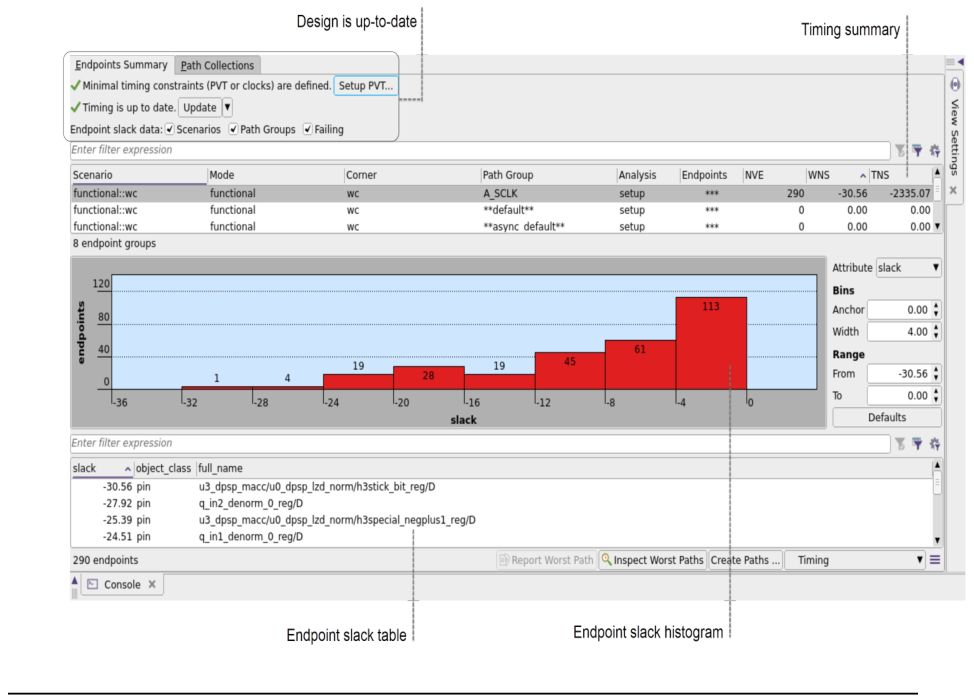
\includegraphics[width=0.92\textwidth]{gui-fig-124.png}
\caption{时序分析摘要窗口}
\label{fig:gui-124}
\end{figure}

\section{创建路径集合}
\subsection*{Creating Path Collections}

在 Timing Analysis 窗口的 Endpoints Summary 选项卡中，可以创建路径集合来选择要分析的路径。在窗口底部的 Endpoint Slack Table 中选择端点，再选择 Create Paths，见图~\ref{fig:gui-125}。

\begin{figure}[htbp]
\centering
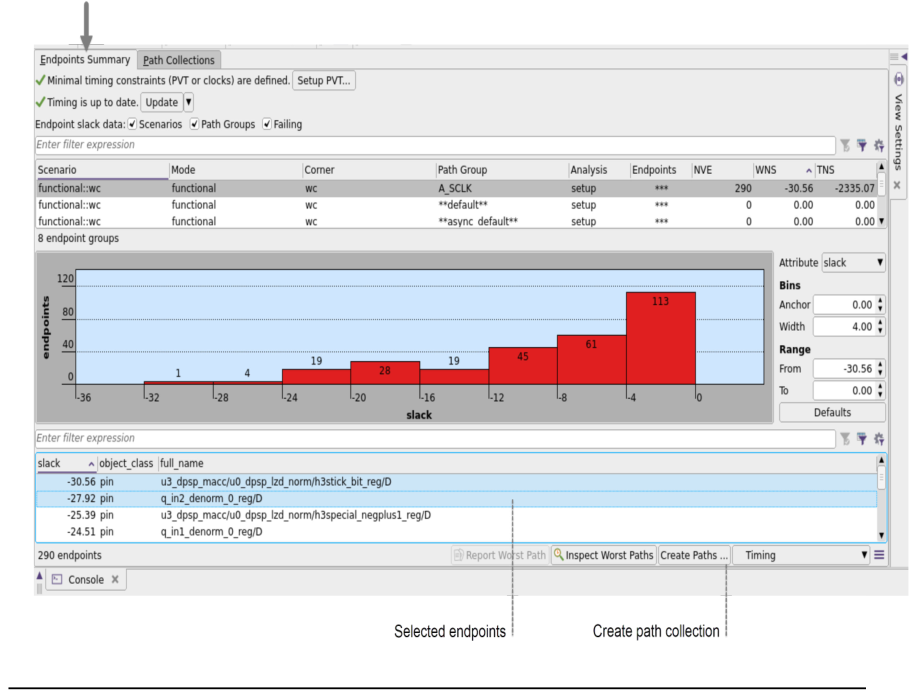
\includegraphics[width=0.92\textwidth]{gui-fig-125.png}
\caption{创建路径集合}
\label{fig:gui-125}
\end{figure}

\subsection{获取时序路径}
\subsubsection*{Getting Timing Paths}

单击 Create Paths 后出现 Get Timing Paths 对话框，见图~\ref{fig:gui-126}。

\begin{figure}[htbp]
\centering
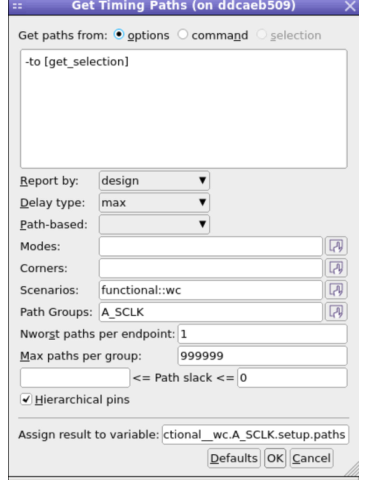
\includegraphics[width=0.8\textwidth]{gui-fig-126.png}
\caption{Get Timing Paths 对话框}
\label{fig:gui-126}
\end{figure}

在该对话框中填写选项，按设计、组、场景（scenario）、模式（mode）或 corner 报告路径。单击 OK 后，端点摘要以直方图显示。要对显示的端点摘要做逻辑级数分析，从下拉菜单选择 logic\_levels，见图~\ref{fig:gui-127}。

\begin{figure}[htbp]
\centering
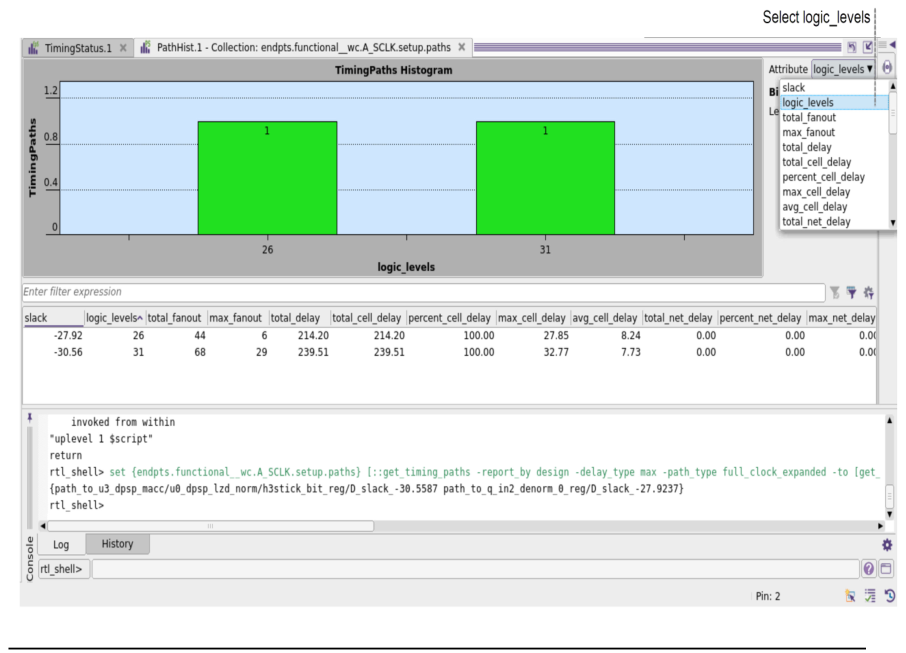
\includegraphics[width=0.85\textwidth]{gui-fig-127.png}
\caption{选择逻辑级数分析}
\label{fig:gui-127}
\end{figure}

\subsection{保存与加载时序路径数据}
\subsubsection*{Saving and Loading Timing Path Data}

要把所选时序路径集合存盘，在 Timing Analysis 窗口底部（Path Collections 选项卡）单击 Write。若保存时启用了片上参数变化（POCV），POCV 数据会与时序路径一起保存。要加载先前保存的数据，单击 Read。若已启用 POCV 且文件中含有 POCV 数据，加载时会一并恢复。

\section{分析时序路径集合}
\subsection*{Analyzing Timing Path Collections}

路径分析器（path analyzer）按你指定的规则分析一组时序路径，根据可用属性值分类，并在按颜色编码的 treemap 中显示各类。可以选择预定义分类规则，或定义自定义规则，也可以添加子类。

在时序分析窗口中选择 \textbf{View > New Path Analyzer} 打开路径分析器。

必须先加载并分类时序路径，才能在 treemap 中查看。

加载一组时序路径：
\begin{enumerate}
  \item 在 Collections 框中指定集合。可以输入集合名，或输入一条创建该集合的 Tcl 命令。
  \item 单击 Apply。
\end{enumerate}

对时序路径分类：
\begin{enumerate}
  \item 在分类树中选择 All。
  \item 单击 Create。出现 Create Category 对话框。
  \item 选择一条规则。
  \item 单击 OK。
\end{enumerate}

可以从同一设计加载一组或多组时序路径。

分类之后，选择分类树顶部的 All，并拖动右侧滑块，在 treemap 中查看各类。All 包含已载入路径分析器的全部路径。

\section{分析逻辑级数}
\subsection*{Analyzing Logic Levels}

在 GUI 中做逻辑级数分析时，路径集合窗口会更新时序路径的直方图，见图~\ref{fig:gui-128}。

\begin{figure}[htbp]
\centering
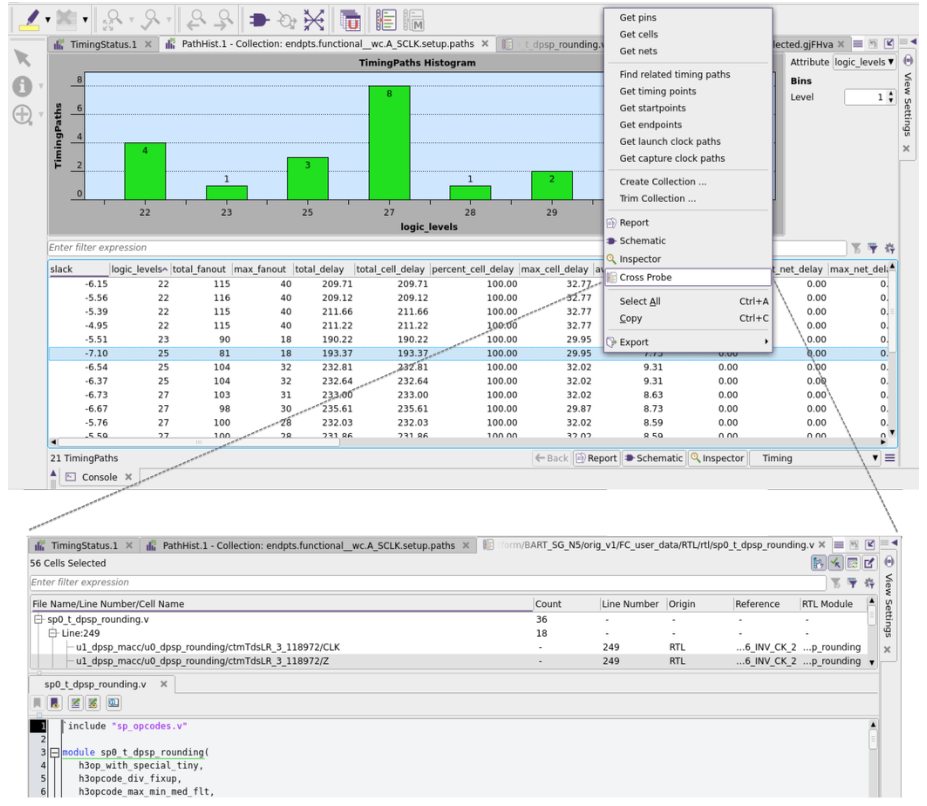
\includegraphics[width=0.92\textwidth]{gui-fig-128.png}
\caption{带逻辑级数的路径集合窗口}
\label{fig:gui-128}
\end{figure}

在端点裕量表中选中一条路径后打开上下文菜单，可以进一步查看，例如显示所选路径的原理图，或用 Cross Probe 显示对应的 RTL。相关入口见图~\ref{fig:gui-129}。

\begin{figure}[htbp]
\centering
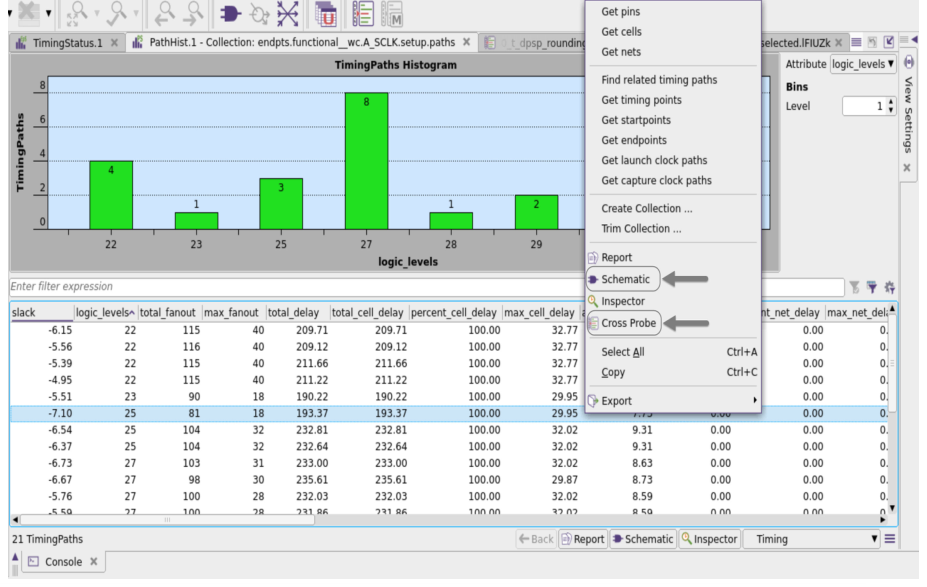
\includegraphics[width=0.7\textwidth]{gui-fig-129.png}
\caption{进一步分析的入口}
\label{fig:gui-129}
\end{figure}
